\section{Logical Volume Management}
\label{section:background-lvm}

Logical Volume Management enables combining multiple individual hard drives and
disk partitions into a single volume group (VG). That volume group can then be
subdivided into logical volumes (LV) or used as a single large volume. Regular
file systems, such as EXT3 or EXT4, can then be created on a logical volume.


Logical volume manager (LVM) introduces an extra layer between the physical
disks and the file system, allowing file systems to:
\begin{itemize}
      \tightlist
      \item
            Be resized and moved with ease and online without requiring a
            system-wide outage.
      \item
            Use discontinuous space on disk.
      \item
            Have meaningful names to volumes, rather than the usual cryptic
            device names.
      \item
            Span multiple physical disks.
\end{itemize}

\begin{figure}[ht]
      \centering
      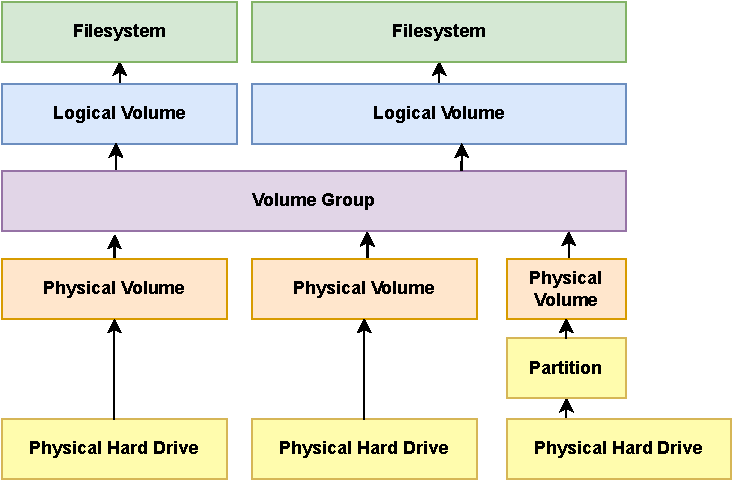
\includegraphics[width=0.8\textwidth]{resources/lvm.pdf}
      \caption{The Logical Volume Management layers}
\end{figure}

The Logical Volume Management consists of the following conceptual layers:
\begin{itemize}
      \item
            \textbf{Physical Volume}: Each Physical Volume can be a disk
            partition, whole disk, meta-device, or a loopback file.
      \item
            \textbf{Volume Group} (VG): A Volume Group gathers a collection of
            Logical Volumes and Physical Volumes into one administrative unit. A
            volume group is divided into fixed-size physical extents. VGs are
            made up of Physical Volumes, which, in turn, are made up of
            physical extents (PEs).

      \item
            \textbf{Logical Volume} (LV): A Logical Volume is the conceptual
            equivalent of a disk partition in a non-LVM system. Logical volumes
            are block devices that are created from the physical extents present
            in the same volume group.
\end{itemize}
